\documentclass[11pt,a4paper]{jsarticle}

\input{include/macro.tex}
\input{include/preamble.tex}

\begin{document}

\section{ソフトウェア} \setcounters{0}

\subsection{アルゴリズム}
  % カメラがポールっぽい物体を捉えていたらそれに向かうベクトルを,
  % なければ総移動距離から自己位置を推定し,予め決められたゴールへ向かうベクトルを採用.
  % 機体周囲に放射状に取り付けた測距センサから適当にベクトルを作って合成.
  % 機体正面に取り付けられた測距センサ三人衆から適当にベクトルを作って合成.
  % ベクトルを適当に左右のモータへの速度指令値(正確にはPWM信号値)に変換して突っ込む.

  \begin{eqnarray}
    \bm{u}_0 = \begin{bmatrix} -0.707 \\ -0.707 \end{bmatrix}, \hspace{5mm} \nonumber
    \bm{u}_1 = \begin{bmatrix}  0     \\ -1     \end{bmatrix}, \hspace{5mm}
    \bm{u}_2 = \begin{bmatrix}  0.707 \\ -0.707 \end{bmatrix}, \hspace{5mm}
    \bm{u}_3 = \begin{bmatrix}  1     \\  0     \end{bmatrix}, \hspace{5mm} \\[3mm]
    \bm{u}_4 = \begin{bmatrix}  0.707 \\  0.707 \end{bmatrix}, \hspace{5mm} \nonumber
    \bm{u}_5 = \begin{bmatrix}  0     \\  1     \end{bmatrix}, \hspace{5mm}
    \bm{u}_6 = \begin{bmatrix} -0.707 \\  0707  \end{bmatrix}, \hspace{5mm}
    \bm{u}_7 = \begin{bmatrix} -1     \\  0     \end{bmatrix}  \hspace{5mm} \\ \nonumber
  \end{eqnarray}

  \begin{figure}[b]
    \begin{center}
      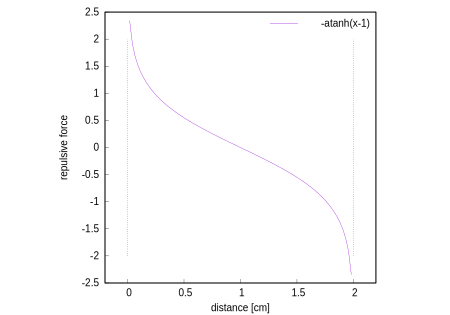
\includegraphics[width=1.0\hsize]{plot/minus_atanh.eps}
    \end{center}
    \caption{ほげほげ}
    \label{fig::atanh}
  \end{figure}

\subsection{画像認識}
  炎上ポールの認識には配布されたRapspberry Pi NoIR Camera V2(以下,カメラモジュール)を使用する.
  画像撮影から最も近い(と思われる)ポールへのベクトルを出力する一連の手順を,簡単に以下に示す.

  \begin{description}
    \item[画像取得] \mbox{} \\
      カメラモジュールへのアクセスには既成ライブラリ\cite{raspicam}を利用した.
      撮影によりピクセル値の二次元配列(cv::Mat)が出力として得られる.
      画像サイズの大小が及ぼす処理時間への影響は極めて大きいが,
      それが画像処理結果の精度に与える影響は未検証であるため,
      現在は適当な値が設定されている.\\
    \item[カラーモデル変換] \mbox{} \\
      得られた画像のカラーモデルをRGBからHSVに変更する.\\
    \item[2値画像化] \mbox{} \\
      HSV画像データに対し赤色マスクをかけて二値画像に変換する.
      赤色マスクの範囲は適当.\\
    \item[ノイズ除去] \mbox{} \\
      適当に膨張・縮小を繰り返してノイズを除去する.
      ちゃんとやってる処理じゃねえから現状ほとんど意味がねえ.\\
    \item[構造解析] \mbox{} \\
      2値画像中の輪郭線を検出した後,それを矩形で囲む.
      囲んだ矩形を縦横比で解析し,ポールの縦横比に対して$\pm 20 \%$以上の差があるものを除外する.
      残った矩形の重心点を求めて,適当にベクトルを作る.\\
  \end{description}

\begin{thebibliography}{9}
  \bibitem{raspicam} "RaspiCam: C++ API for using Raspberry camera with/without OpenCV",\\
                     "\texttt{https://www.uco.es/investiga/grupos/ava/node/40}",2017年5月31日最終確認.
\end{thebibliography}

\end{document}
